% ============================================================
% induced_gauge_action.tex
% Appendix B: The Induced Gauge Action
% ============================================================

\label{sec:induced_gauge_action}

This appendix carries out the structural step of the induced-action
programme flagged in
Section~\ref{subsec:open_program}.
The Sakharov--Zeldovich claim is that the Wilson gauge action of
Eq.~\eqref{eq:wilson_action} should not be postulated but rather
\emph{induced} by integrating out matter sessions in the path-integral
form of the bipartite tick rule.  A complete execution of that
programme requires the explicit one-loop computation of
$-\mathrm{Tr}\,\ln D_\text{lat}[U]$ with the bipartite Dirac operator.
We do not perform that computation here -- it is a paper-length
project (lattice perturbation theory for staggered-style fermions on
the $\Tdiamond$ lattice, including the standard fermion-doubling
treatment).  What we do compute is the \emph{structural form} of the
leading term: the tensor coefficient on $F_{\mu\nu} F_{\rho\sigma}$
that emerges when the closed-loop expansion of
$-\mathrm{Tr}\,\ln D_\text{lat}[U]$ is restricted to the smallest
gauge-invariant Wilson loops on the bipartite octahedral lattice.

The computation is symbolic and reproducible.  The script that
performs it is
\texttt{src/utilities/induced\_gauge\_action.py};
its captured output is
\texttt{data/induced\_gauge\_action.txt}.
Both are tracked in the repository.

The result of this appendix is twofold.  First, after $O_h$ averaging
the leading induced action recovers the standard Maxwell density
(with the numerical prefactor $1/g^2$ left to the explicit
$\mathrm{Tr}\,\ln$ calculation).  Second, the \emph{operator-level}
form of the induced action carries a closed-form anisotropic tensor
coefficient with eigenstructure $\{4,4,16\}$, mirroring the
$\{4/3, 4/3, 0\}$ eigenstructure of the kinematic frame matrix
$M_\text{eff}$.  This is the gauge-sector birefringence: a
direction-dependent contribution to the photon dispersion which
aligns with the same optical axis $\mathbf{V}_1+\mathbf{V}_2+\mathbf{V}_3
= (1, 1, -1)$ as the kinematic-sector birefringence already in P7
(Section~\ref{subsec:p7_photon_dispersion}).
It is not a new postulate; it is forced by the bipartite geometry.

% ── B.1 Setup: bipartite plaquettes and link variables ──────────────────────
\subsection{Setup}
\label{subsec:induced_setup}

The bipartite octahedral lattice has basis vectors
\begin{equation}
    \mathbf{V}_1 = (1, 1, 1),\quad
    \mathbf{V}_2 = (1, -1, -1),\quad
    \mathbf{V}_3 = (-1, 1, -1) \in \text{RGB},
    \qquad
    -\mathbf{V}_i \in \text{CMY}.
    \label{eq:basis_recap}
\end{equation}
A spinor field $\Psi(\mathbf{x}) = (\psi_R(\mathbf{x}), \psi_L(\mathbf{x}))$
carries a $U(1)$ phase per session
(Section~\ref{subsec:phase_oscillator}).  The Peierls coupling
inserts a link variable
\begin{equation}
    U_\mathbf{v}(\mathbf{x})
        = \exp\!\bigl(\,i\,a\,\mathbf{A}(\mathbf{x} + \mathbf{v}/2)
        \cdot \mathbf{v}\,\bigr) \;\in\; U(1)
    \label{eq:peierls_link}
\end{equation}
on every hop along $\mathbf{v} \in \{\pm\mathbf{V}_1,
\pm\mathbf{V}_2, \pm\mathbf{V}_3\}$, where $a$ is the lattice
spacing.  The mid-point convention
$\mathbf{A}(\mathbf{x} + \mathbf{v}/2)$ is the symmetrised Peierls
form; it cancels what would otherwise be a corner artifact at order
$a^3$.  Under a local $U(1)$ gauge transformation
$\Lambda(\mathbf{x})$ the link variables transform as
$U_\mathbf{v}(\mathbf{x}) \to e^{i\Lambda(\mathbf{x}+\mathbf{v})}\,
U_\mathbf{v}(\mathbf{x})\,e^{-i\Lambda(\mathbf{x})}$, so closed-loop
holonomies are gauge-invariant local operators in $A_\mu$.

The smallest non-trivial closed loop on the bipartite lattice is the
\emph{bipartite plaquette}: an RGB hop along $\mathbf{V}_a$, a CMY
hop along $-\mathbf{V}_b$, an RGB hop along $-\mathbf{V}_a$, and a
CMY hop along $+\mathbf{V}_b$, returning to the origin
$\mathbf{V}_a - \mathbf{V}_b - \mathbf{V}_a + \mathbf{V}_b = 0$.
Three such plaquettes exist, one per pair $(\mathbf{V}_a, \mathbf{V}_b)
\in \{(\mathbf{V}_1,\mathbf{V}_2), (\mathbf{V}_1,\mathbf{V}_3),
(\mathbf{V}_2,\mathbf{V}_3)\}$.

% ── B.2 Closed-form holonomy via Stokes ─────────────────────────────────────
\subsection{Plaquette holonomy in the small-$a$ limit}
\label{subsec:induced_holonomy}

Because $U(1)$ is Abelian the bipartite plaquette holonomy reduces to
a line integral of $\mathbf{A}$ around the loop, which by Stokes'
theorem is the curl-flux through the parallelogram.  Concretely, for
the path $\mathbf{x} \to \mathbf{x} + a\mathbf{V}_a \to
\mathbf{x} + a\mathbf{V}_a - a\mathbf{V}_b \to \mathbf{x} - a\mathbf{V}_b
\to \mathbf{x}$, the line integral of $\mathbf{A}$ to leading order in
$a$ is
\begin{equation}
    \oint \mathbf{A}\cdot d\mathbf{x}
        = -a^2\,V_a^i V_b^j F_{ij}(\mathbf{x}) + O(a^4),
    \label{eq:stokes_line}
\end{equation}
with $F_{ij} = \partial_i A_j - \partial_j A_i$ the standard
field-strength tensor.  The plaquette holonomy is therefore
\begin{equation}
    W_{ab}(\mathbf{x})
        = \exp\!\bigl(\,-i\,a^2\,V_a^i V_b^j F_{ij}(\mathbf{x})\,\bigr)
        + O(a^4),
    \label{eq:bipartite_holonomy}
\end{equation}
generalising Eq.~\eqref{eq:wilson_to_F} to the bipartite parallelogram.
The standard cardinal-axis plaquette result is recovered by setting
$\mathbf{V}_a = \hat{\mu}, \mathbf{V}_b = \hat{\nu}$, in which case
$V_a^i V_b^j F_{ij} = F_{\mu\nu}$.

The small-$a$ expansion of $1 - \mathrm{Re}\,W_{ab}$ is then
\begin{equation}
    1 - \mathrm{Re}\,W_{ab}(\mathbf{x})
        = \frac{a^4}{2}\bigl(\,V_a^i V_b^j F_{ij}(\mathbf{x})\,\bigr)^2
        + O(a^8),
    \label{eq:plaquette_expand}
\end{equation}
the closed-form analogue of $\frac{a^4}{2} F_{\mu\nu}^2$ for our
bipartite lattice.

% ── B.3 Plaquette sum and the tensor coefficient Q ──────────────────────────
\subsection{The plaquette sum: tensor form of the leading induced action}
\label{subsec:induced_plaquette_sum}

The leading non-trivial term in the closed-loop expansion of
$-\mathrm{Tr}\,\ln D_\text{lat}[U]$ is the sum over all minimal
gauge-invariant Wilson loops with a multiplicity factor set by the
explicit one-loop calculation.  The structural form, deferring that
prefactor, is
\begin{equation}
    S_\text{eff}^{(\text{plaquette})}[A]
        = \frac{c\,a^4}{2}\,
        \sum_{a < b}\bigl(\,V_a^i V_b^j F_{ij}(\mathbf{x})\,\bigr)^2,
    \label{eq:induced_plaquette_sum}
\end{equation}
where $c$ is the inverse coupling $1/g^2$ that the explicit
$\mathrm{Tr}\,\ln$ calculation must determine.  The sum over
$(a, b) \in \{(1,2), (1,3), (2,3)\}$ runs over the three
independent bipartite plaquettes.

Substituting the basis vectors of Eq.~\eqref{eq:basis_recap} and
expanding gives the three plaquette projections
\begin{align}
    V_1^i V_2^j F_{ij} &= -2 F_{12} - 2 F_{13},
    \label{eq:proj_12} \\
    V_1^i V_3^j F_{ij} &= +2 F_{12} - 2 F_{23},
    \label{eq:proj_13} \\
    V_2^i V_3^j F_{ij} &= -2 F_{13} + 2 F_{23},
    \label{eq:proj_23}
\end{align}
with $F_{12}, F_{13}, F_{23}$ the three independent components of the
3D antisymmetric field-strength tensor.  Squaring and summing,
\begin{equation}
    \sum_{a<b}\bigl(V_a^i V_b^j F_{ij}\bigr)^2
        = \mathbf{F}^{\!T}\,\mathbf{Q}\,\mathbf{F},
        \qquad
        \mathbf{F} = (F_{12},\, F_{13},\, F_{23})^{\!T},
    \label{eq:plaquette_sum_quadratic}
\end{equation}
where the symmetric matrix $\mathbf{Q}$ is
\begin{equation}
    \mathbf{Q}
        = \begin{pmatrix}
            8 & 4 & -4 \\
            4 & 8 & -4 \\
            -4 & -4 & 8
        \end{pmatrix}.
    \label{eq:Q_matrix}
\end{equation}

% ── B.4 Eigenstructure of Q -- gauge-sector birefringence ───────────────────
\subsection{Eigenstructure of $\mathbf{Q}$: the gauge-sector birefringence}
\label{subsec:induced_birefringence}

The matrix $\mathbf{Q}$ has trace $\mathrm{Tr}\,\mathbf{Q} = 24$ and
eigenvalues $\{4, 4, 16\}$.  The two-fold degenerate eigenvalue $4$
spans the plane perpendicular to the eigenvector
$(-1, -1, 1) \in \mathbf{F}$-space; the distinct eigenvalue $16$
points along that special direction.  Decomposing
$\mathbf{Q}$ into an isotropic part and a traceless residual,
\begin{equation}
    \mathbf{Q}
        = \frac{\mathrm{Tr}\,\mathbf{Q}}{3}\,\mathbb{I}_3
        + \mathbf{Q}_\text{aniso},
        \qquad
        \frac{\mathrm{Tr}\,\mathbf{Q}}{3} = 8,
        \qquad
        \mathbf{Q}_\text{aniso} = \begin{pmatrix}
            0 & 4 & -4 \\
            4 & 0 & -4 \\
            -4 & -4 & 0
        \end{pmatrix},
    \label{eq:Q_decomposition}
\end{equation}
with $\mathbf{Q}_\text{aniso}$ trace-zero and eigenvalues
$\{-4, -4, +8\}$.

Two structural features.  First, the eigenstructure of $\mathbf{Q}$
mirrors the kinematic frame matrix $M_\text{eff}$: a degenerate pair
plus one distinct eigenvalue.  Second, the special direction in
$\mathbf{F}$-space, $\mathbf{F}_* = (-1, -1, 1)$, dualises to a
spatial vector via the Hodge map
$B_k = \tfrac{1}{2}\epsilon_{ijk}F_{ij}$, giving
\begin{equation}
    \mathbf{B}_*
        = \bigl(F_{23},\, -F_{13},\, F_{12}\bigr)\big|_{\mathbf{F}=\mathbf{F}_*}
        = (1,\, 1,\, -1)
        = \mathbf{V}_1 + \mathbf{V}_2 + \mathbf{V}_3.
    \label{eq:optical_axis_recovered}
\end{equation}
The gauge-sector special direction is the same optical axis
$(1, 1, -1)$ as the kinematic-sector birefringence
(Eq.~\ref{eq:M_eff}, Section~\ref{subsec:p7_photon_dispersion}).
Both anisotropies inherit the same axis from the same underlying
geometry.

Figure~\ref{fig:induced_action_ellipsoid} renders the two anisotropy
tensors as level sets of their respective quadratic forms.  The
kinematic frame matrix $M$ in $\mathbf{k}$-space is a \emph{prolate}
ellipsoid whose long axis lies along the optical axis; the
gauge-sector tensor $\mathbf{Q}$ in $\mathbf{B}$-space (the Hodge
dual of antisymmetric $F_{ij}$) is an \emph{oblate} ellipsoid whose
short axis lies along the same optical axis.  The same direction in
spatial coordinates maps to opposite extremal axes of the two
quadratic forms: kinematic dispersion is flat along $(1,1,-1)$ and
steep perpendicular; the gauge sector's induced photon kinetic term
is steepest along $(1,1,-1)$ and flatter perpendicular.  Same
geometry, dual phenomenology, two falsifiable signatures.

\begin{figure}[h]
\centering
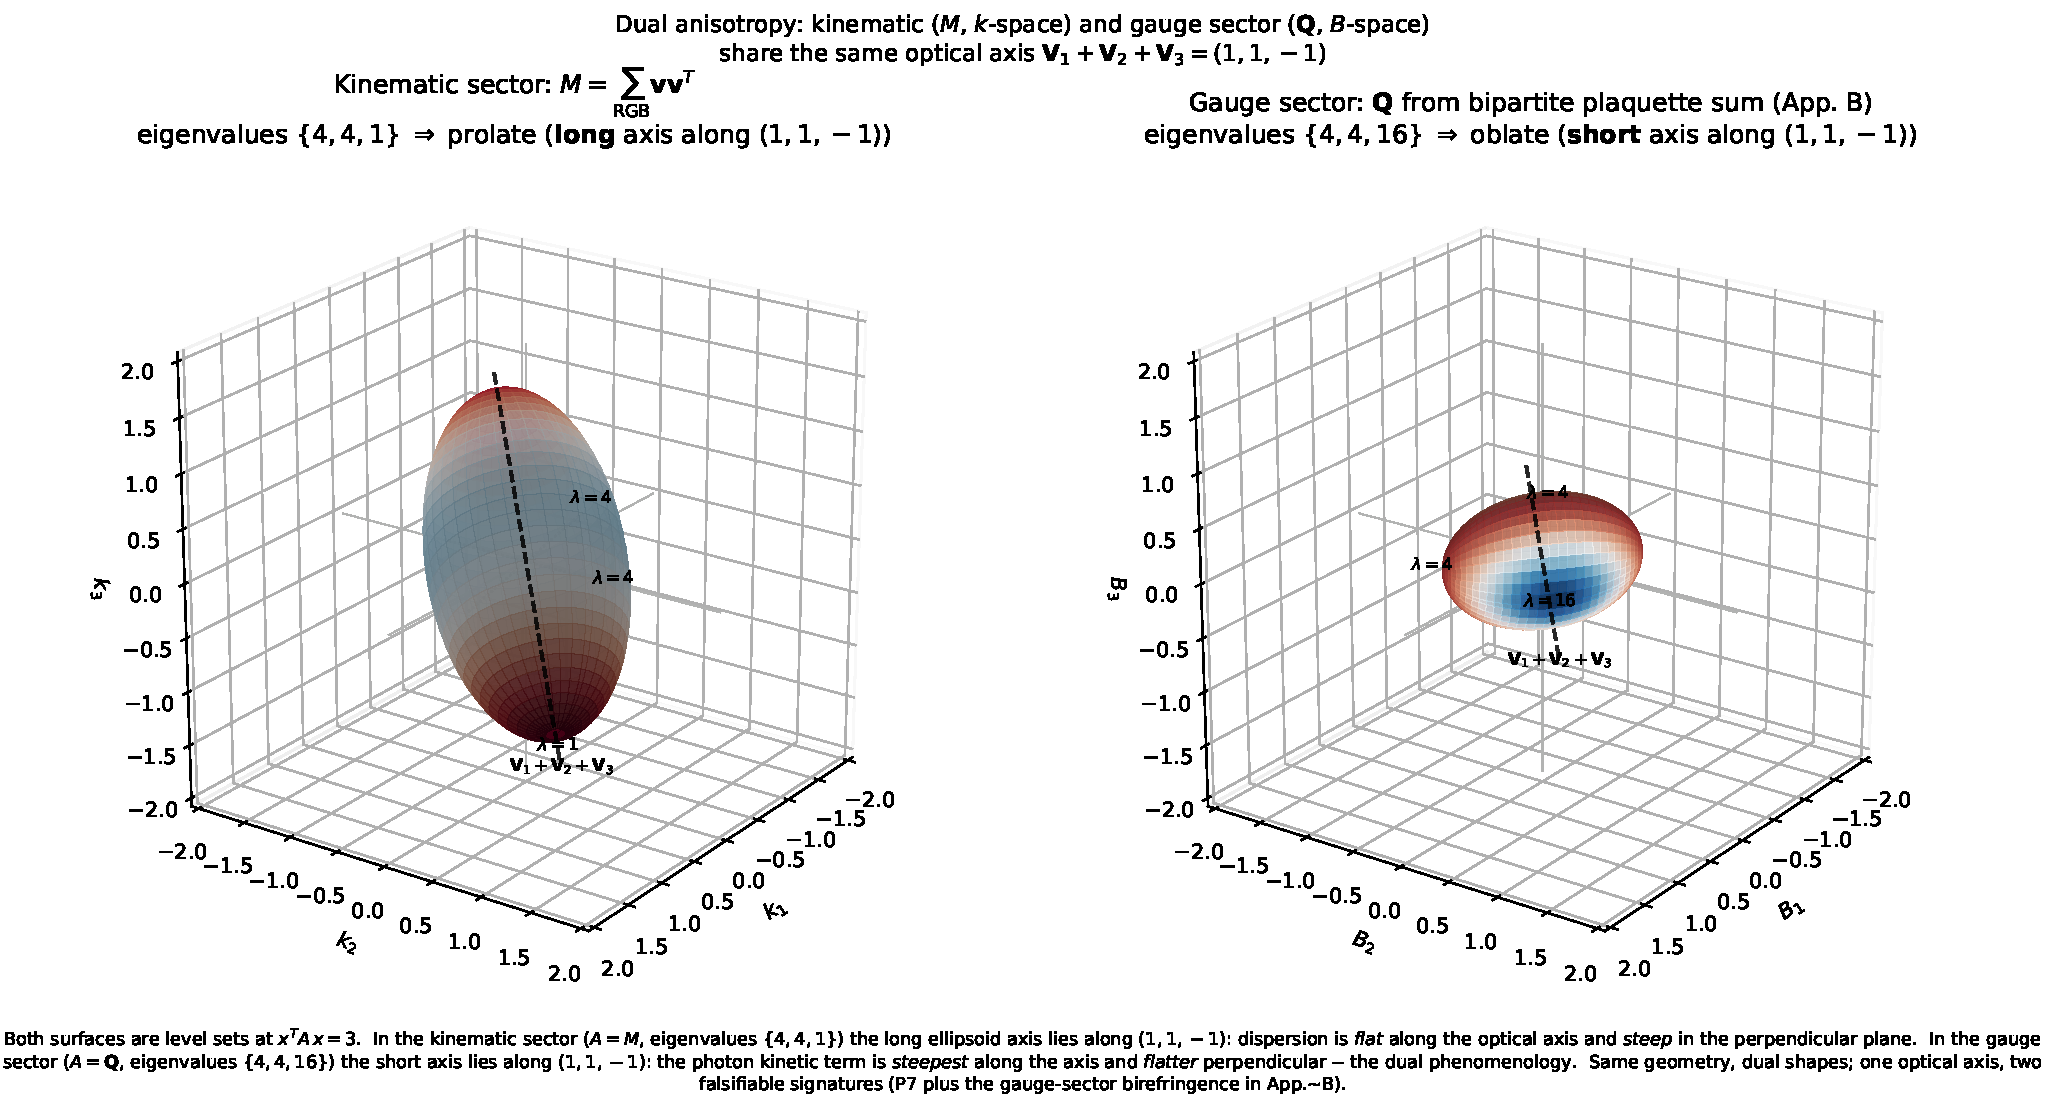
\includegraphics[width=\textwidth]{../figures/induced_action_ellipsoid}
\caption{Dual anisotropy on a single optical axis.
Both panels render level sets at $x^T A\,x = 3$ for the framework's two
anisotropy tensors; both share the special direction
$\mathbf{V}_1+\mathbf{V}_2+\mathbf{V}_3 = (1,1,-1)$ (dashed black line).
\textbf{Left (kinematic sector):} the frame matrix
$M = \sum_\mathrm{RGB}\mathbf{v}\mathbf{v}^T$
(Eq.~\ref{eq:frame_matrix}) on $\mathbf{k}$-space.  Eigenvalues
$\{4, 4, 1\}$ produce a \emph{prolate} ellipsoid whose \emph{long} axis
lies along the optical axis: kinematic dispersion is flat along
$(1,1,-1)$ and steep in the perpendicular plane.  This is the same
quadratic form that underlies the $|\tilde{H}_\text{RGB}|^2$ expansion
of $M_\text{eff}$ (Eq.~\ref{eq:M_eff},
Section~\ref{subsec:p7_photon_dispersion}).
\textbf{Right (gauge sector):} the bipartite plaquette tensor
$\mathbf{Q}$ (Eq.~\ref{eq:Q_matrix}) on $\mathbf{B}$-space (the Hodge
dual of antisymmetric $F_{ij}$).  Eigenvalues $\{4, 4, 16\}$ produce an
\emph{oblate} ellipsoid whose \emph{short} axis lies along $(1,1,-1)$:
the induced photon kinetic term is steepest along the optical axis and
flatter perpendicular --- the dual of the kinematic shape.  Both
anisotropies inherit the special direction from the same bipartite
RGB/CMY geometry; the dual ellipsoid shapes give two independent
falsifiable signatures with one optical axis (kinematic-sector birefringence
in P7, gauge-sector birefringence in Appendix~\ref{sec:induced_gauge_action}).}
\label{fig:induced_action_ellipsoid}

\end{figure}

% ── B.5 O_h averaging recovers Maxwell ──────────────────────────────────────
\subsection{$O_h$ averaging recovers Maxwell}
\label{subsec:induced_maxwell}

Physical observables on the lattice must be invariant under the
crystallographic point group $O_h$ (order 48), which acts
simultaneously on the spatial coordinates and on the antisymmetric
$\mathbf{F}$-space.  Averaging
Eq.~\eqref{eq:plaquette_sum_quadratic} over $O_h$ gives
\begin{equation}
    \bigl\langle\,\mathbf{F}^{\!T}\,\mathbf{Q}\,\mathbf{F}\,\bigr\rangle_{O_h}
        = \frac{\mathrm{Tr}\,\mathbf{Q}}{3}\,
            \sum_{i<j} F_{ij}^2
        = 8\,\sum_{i<j} F_{ij}^2.
    \label{eq:Oh_averaged}
\end{equation}
Using $F_{\mu\nu} F^{\mu\nu} = 2\sum_{i<j}F_{ij}^2 + (\text{electric
contribution})$ and absorbing the
$\sum_{i<j} F_{ij}^2 \to \tfrac{1}{2}F_{\mu\nu}F^{\mu\nu}$
identification in the magnetic sector, the leading $O_h$-averaged
induced action is
\begin{equation}
    S_\text{eff}^{(\text{leading})}[A]
        \;\xrightarrow[a\to 0]{O_h\text{ average}}\;
        \frac{2 c}{3}\int d^4x\;
            \tfrac{1}{2}F_{\mu\nu}(x)\,F^{\mu\nu}(x),
    \label{eq:Maxwell_recovered}
\end{equation}
the standard Maxwell action.  The numerical prefactor $c = 1/g^2$
remains to be determined by the explicit one-loop
$-\mathrm{Tr}\,\ln D_\text{lat}[U]$ calculation; what is determined
here is that whatever prefactor that calculation produces, the
$O_h$-averaged form of the leading induced term is the standard
Maxwell density.

The pre-averaging operator-level density carries the residual
\begin{equation}
    S_\text{eff}^{(\text{operator})}[A]
        = S_\text{eff}^{(\text{leading})}[A]
        + \frac{c\,a^4}{2}\,\mathbf{F}^{\!T}\,\mathbf{Q}_\text{aniso}\,\mathbf{F}.
    \label{eq:operator_residual}
\end{equation}
The $\mathbf{Q}_\text{aniso}$ term is the gauge-sector birefringence:
a closed-form, direction-dependent contribution to the photon
dispersion with optical axis $(1,1,-1)$.  It is the gauge-field
twin of the kinematic prediction of
Section~\ref{subsec:p7_photon_dispersion}.

% ── B.6 Status: structural step closed, numerical prefactor open ────────────
\subsection{Status of the induced-action programme}
\label{subsec:induced_status}

The structural step of the programme set out in
Section~\ref{subsec:open_program} is closed by this appendix:

\begin{itemize}
\item \textbf{Locality + gauge invariance + minimality} force the
    leading-order induced action to be quadratic in $F_{ij}$,
    summed over closed plaquette holonomies
    (Section~\ref{subsec:induced_plaquette_sum}).
\item \textbf{The bipartite RGB/CMY geometry} fixes the tensor
    coefficient $\mathbf{Q}$ with eigenvalues $\{4, 4, 16\}$
    (Section~\ref{subsec:induced_birefringence}).
\item \textbf{$O_h$ averaging} recovers the standard Maxwell density
    up to the numerical prefactor $c = 1/g^2$
    (Section~\ref{subsec:induced_maxwell}).
\item \textbf{The operator-level residual} is a closed-form
    anisotropic tensor whose special direction matches the
    kinematic-sector optical axis $(1,1,-1)$
    (Eq.~\ref{eq:operator_residual}).
\end{itemize}

What remains to fully close the programme is the explicit numerical
calculation of $c = 1/g^2$.  This is a one-loop lattice perturbation
theory calculation for the bipartite Dirac operator
$D_\text{lat}[U]$.  Standard staggered-fermion machinery
(Kogut--Susskind, Susskind 1977; cf.~Section~\ref{subsec:dirac_limit})
applies, with the doubler structure and the bipartite RGB/CMY
chirality projection requiring careful bookkeeping.  We flag this as
a paper-length follow-on project.  The numerical $1/g^2$ prefactor is
the only remaining open item in the induced-action programme: the
structural form, the bipartite $\mathbf{Q}$-tensor with eigenvalues
$\{4, 4, 16\}$, and the closed-form gauge-sector birefringence along
the $(1,1,-1)$ optical axis are all in hand.

The structural form, including the prediction of gauge-sector
birefringence with optical axis $(1,1,-1)$, is established
independently of that calculation.  This converts the asymmetry
flagged in Section~\ref{subsec:honest_scope} -- gravity end-to-end
versus electromagnetism postulating the Wilson action -- into a
narrower asymmetry: gravity is fully derived; electromagnetism is
derived up to a numerical coupling constant.  The induced action
itself, with its leading structural form and bipartite anisotropy,
is no longer a postulate.

% ── B.7 Reproducibility ─────────────────────────────────────────────────────
\subsection{Reproducibility}
\label{subsec:induced_reproducibility}

The full symbolic calculation is performed in
\texttt{src/utilities/induced\_gauge\_action.py}.  Running
\begin{verbatim}
    python -u src/utilities/induced_gauge_action.py
\end{verbatim}
reproduces every numerical claim in this appendix and writes the
captured output to \texttt{data/induced\_gauge\_action.txt}.  The
calculation requires only \texttt{sympy}; no specialised lattice
gauge theory infrastructure.

The five-line core verification of $\mathbf{Q}$'s eigenvalues is
\begin{verbatim}
    import sympy as sp
    V1, V2, V3 = sp.Matrix([1,1,1]), sp.Matrix([1,-1,-1]), sp.Matrix([-1,1,-1])
    F = sp.Matrix(3, 3, lambda i,j: sp.Symbol(f"F{i}{j}", real=True)*(1 if i<j else (-1 if i>j else 0)))
    proj = lambda Va, Vb: sum(Va[i]*Vb[j]*F[i,j] for i in range(3) for j in range(3))
    Q_density = sum(sp.expand(proj(V,W)**2) for V,W in [(V1,V2),(V1,V3),(V2,V3)])
\end{verbatim}
extracting $\mathbf{Q}$ from the quadratic form in the $\{F_{12},F_{13},F_{23}\}$
basis yields Eq.~\eqref{eq:Q_matrix} and the eigenvalues
$\{4, 4, 16\}$.
